\subsubsection{Aufgabe der Komponente}
Durch das Radar können Geräte, auf welchen ebenfalls die Anwendung SharkNet installiert ist, in räumlicher Nähe ausfindig gemacht und angezeigt werden. Es nutzt dabei die Verhaltensweise der WiFi-Komponente, bei der in regelmäßigen Abständen Ge\-rä\-te\-in\-for\-ma\-tio\-nen an alle Geräte in der Nähe geschickt werden. Diese Geräteinformationen werden vom Radar empfangen, gebündelt und dem Benutzer dann auf dem Gerät als Liste angezeigt. Der Benutzer kann anschließend anhand dieser Geräteliste einen Chat eröffnen. Neben der Eröffnung von Chats ist diese Geräteliste außerdem wichtig für die Broadcast-Komponente, da Broadcast Nachrichten an alle Geräte geschickt werden, die sich auf dieser Liste befinden.\newline
\begin{figure}[H]
	\centering
	\makebox[\linewidth][c]{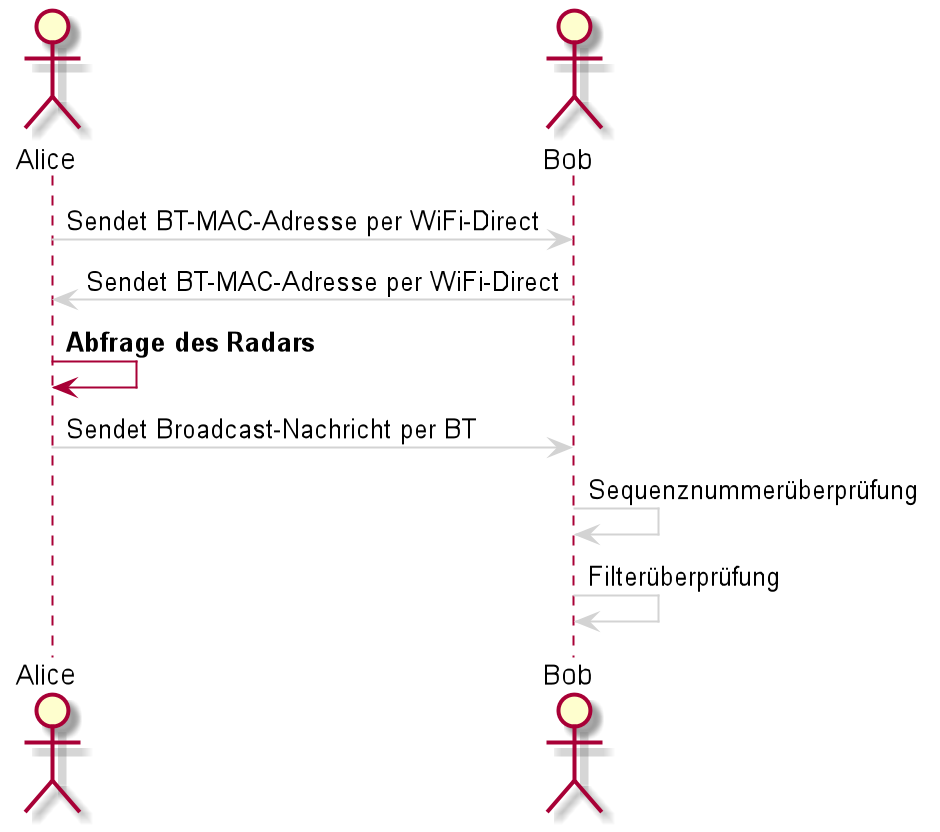
\includegraphics[width=0.6\linewidth]{radar/images/communicationComps.png}}%
	\caption{Die Radar-Komponente innerhalb des Nachrichtenaustauschs}
	\label{fig:radarComp}
\end{figure}
\newpage
\subsubsection{Architektur}

Im folgenden UML-Klassendiagramm sind alle Bestandteile der Radar-Komponente von SharkNet abgebildet:
\begin{figure}[H]
	\centering
	%\hspace*{1cm}
	\scalebox{1}[0.9]{\makebox[\linewidth][c]{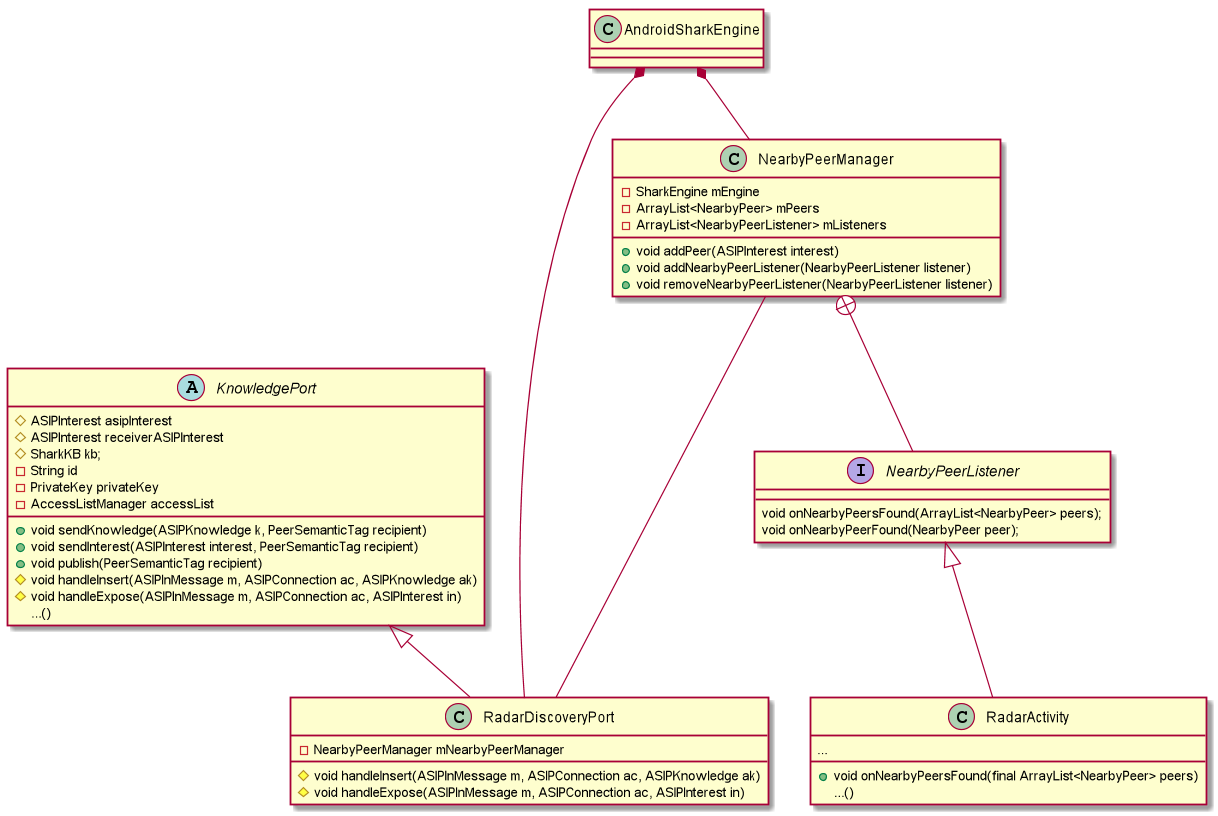
\includegraphics[width=1\linewidth]{radar/images/radar.png}}}
	\caption{Die Radar Klassen im Überblick}
	\label{fig:radarhAll}
\end{figure}
Die eingangs erwähnte Geräteliste befindet sich als Attribut innerhalb der Klasse \textit{Nearby\-Peer\-Manager}. Die Klasse enthält das Interface \textit{NearbyPeerListener}, welches für die Benachrichtigungen im Falle von neu gefundenen Geräten zuständig ist. Android Activities wie die \textit{RadarActivity} oder aber auch die \textit{BroadcastActivity} implementieren dieses Interface, um stets über alle Geräte in der Nähe informiert zu sein. Der \textit{RadarDiscoveryPort} ist die Schnittstelle zwischen Anwendung und Shark Framework. Die im Grundlagenkapitel erwähnten Knowledge-Port-Methoden \textit{handleInsert()} und \textit{handleExpose()} werden benötigt, weil die Geräte ihre Informationen in Form von ASIP-Interessen versenden. Diese Interessen werden nach dem Empfang dann auf der Ebene des Frameworks durch die Methode \textit{handleExpose()} verarbeitet und anschließend auf der Ebene der Anwendung dem Benutzer dargestellt.

\subsubsection{Nutzung}
Die Komponente kann über die \textit{startDiscovery()} Methode der \textit{AndroidSharkEngine} gestartet werden.

\subsubsection{Code}
Wie im Überblick dargestellt werden über Interessen Kontaktinformationen ausgetauscht. Eingehende Interessen werden vom \textit{RadarDiscoveryPort} folgendermaßen bearbeitet:\newline
 \lstset{language=Java, caption=Verwertung von  Kontakt-Interessen (Auszug), label=DescriptiveLabel, numbers=left, numbersep=1em, breaklines=true, basicstyle=\small}
\begin{lstlisting}
protected void handleExpose(ASIPInMessage message, ASIPConnection asipConnection, ASIPInterest interest) throws SharkKBException {
if (interest == null) return;
STSet types = interest.getTypes();
if (types == null || types.isEmpty()) return;
SemanticTag typeSemanticTag = types.getSemanticTag(WifiDirectAdvertisingManager.TYPE_SI);
if (SharkCSAlgebra.identical(message.getTopic(), typeSemanticTag)) {
  mNearbyPeerManager.addPeer(interest);
}
\end{lstlisting}
Sollte das Interesse leer sein (erste Zeile) oder vom Typ her nicht einer Kontaktinformation entsprechen (vierte bis sechste Zeile), wird nichts der Kontaktliste hinzugefügt. Andernfalls (siebte Zeile) wird der Kontaktliste innerhalb des \textit{NearbyPeerManager} der neue Kontakt hinzugefügt und auf der Oberfläche angezeigt. Dadurch hinzugefügte Kontakte können nun Broadcast-Nachrichten empfangen.
\newpage
\subsubsection{Gerätetest}
Mit den folgenden Android-Geräten ist die Komponente auf Kompatibilität geprüft worden:\\
\begin{table}[H]
	\begin{center}
		\begin{tabular}{l|c|c} 			
			Gerät & Android-Version & kompatibel \\
			\hline
			LG Nexus 5x & 8.0 & Ja\\
			LG Nexus 5x & 8.1 & Ja\\
			LG Nexus 5 & 6.1 & Ja\\
			Sony Xperia XZ Premium & 8.0 & Ja\\
			Sony Xperia Z4 Tablet & 7.1.1 & Ja\\
			Lenovo B & 6.0 & Ja\\
			Lenovo A5500-F Tablet & 4.4 & Ja\\
			Raspberry Pi 3 & 6.0.1 & Ja\\	
			Wandboard Quad & 5.0.2 & Ja\\			
		\end{tabular}
		\caption{Kompatibilitätstest der Radar-Komponente}
		\label{tab:dimensions}
	\end{center}
\end{table}
Hierbei ist zu beachten, dass es bei der Komponente vorrangig um die Darstellung und Speicherung der über WiFi-Direct erhaltenen Daten geht. Die benutzten Ober\-flä\-chen\-ele\-mente können von allen getesteten Android-Versionen benutzt werden. Das Radar kann nach aktuellem Stand nicht ohne die WiFi-Komponente ordentlich funktionieren, daher muss auch der Kompatibilitätstest der WiFi-Komponente beachtet werden. Das Radar ist dennoch als eigenständige Komponente ausgeführt, da sie die Kontaktdaten theoretisch auch durch andere Komponenten erhalten könnte.  
\subsubsection{Ausblick}
Das Radar listet die gefundenen Geräte bisher nur in einer Liste auf. Diese könnten in Zukunft auch zusätzlich auf einer Karte angezeigt werden, dadurch wird der aktuelle Ort der anderen Geräte für den Benutzer sichtbar. Außerdem könnten neben dem Namen der Geräte noch zusätzliche Informationen aufgelistet werden. So könnten beispielsweise noch Interessen der Geräte angezeigt werden, dafür müsste jedoch eine geeignete Darstellungsform gefunden werden.
\\Sollten noch zusätzliche Informationen angezeigt werden, muss es für die Benutzer zwingend einstellbar sein, in welchem Ausmaß Kontaktinformationen preisgeben werden.  
\newpage